% small.tex
\documentclass[handout]{beamer}
\usetheme{default}
\usepackage{color}
\usepackage[labelformat=empty]{caption}
\usepackage{amsfonts, amsmath, amsthm, amssymb,epstopdf}

%%% allows color text:
\usepackage{xcolor}

%%% Allows adding "links", i.e url
\usepackage{hyperref}

%\useoutertheme[subsection=false]{smoothbars}
\usetheme{Warsaw}
%\usecolortheme[rgb={0.2,0.3,0.7}]{structure}
%\setbeamercovered{highly dynamic}

\usepackage{amsmath,amssymb,latexsym}


% adding slide numbers
\addtobeamertemplate{navigation symbols}{}{%
    \usebeamerfont{footline}%
    \usebeamercolor[fg]{footline}%
    \hspace{1em}%
    \insertframenumber/\inserttotalframenumber
}
%%%%%%%%%%%%%%%%%%%%%%%%%%%%%%%%%%%%%%%%%%%%%%%%%%

\usepackage[round,sort,longnamesfirst]{natbib}


%%% Details:
\author{Yotam Shem-Tov}
\title{STAT 239/ PS 236A}

\begin{document}
\setbeamertemplate{caption}{\insertcaption}


\begin{frame}{}

\centering

\LARGE

$\bold{Section}$ $\bold{1:}$ $\bold{Regression}$ $\bold{Review}$

\vspace{0.4 in}

\large
\textit{Yotam Shem-Tov}

\vspace{0.1 in}

\textit{Fall 2014}

\end{frame}

%%%%%%%%%%%%%%%%%%%%%%%%%%%%%%%%
%%% Slides: 
%%%%%%%%%%%%%%%%%%%%%%%%%%%%%%%%

\begin{frame}{Contact information}
\begin{itemize}

\item Yotam Shem-Tov, PhD student in economics
\item E-mail: shemtov@berkeley.edu
\item Office hours: Wednesday 2-4
\end{itemize}
\end{frame}


\begin{frame}{}
There are two general approaches to regression \\~\\
\begin{enumerate}
\item Regression as a model: a data generating process (DGP)
\item Regression as an algorithm, i.e as a predictive model \\~\
\end{enumerate}
This two approaches are different, and make different assumptions
\end{frame}

\begin{frame}{Regression as a prediction}
	\begin{itemize}
		\item<+-> We have an input vector $X^T = (X_1, X_2, \dots, X_p)$ with dimensions of  $n \times p$ and an output vector $Y$ with dimensions $n \times 1$. 
		\item<+-> The linear regression model has the form:
		$$ f(X) = \beta_0 + \sum_{j=1}^p X_j \beta_j $$
		\item<+-> We can pick the coefficients $\beta = (\beta_0,\beta_1,\dots,\beta_p)^T$ in a variety of ways but OLS is by far the most common, which minimizes the \textbf{residual sum of squares} (RSS):
		  \begin{align*}
			RSS(\beta) &= \sum_{i=1}^N (y_i - f(x_i))^2 \\
					   &= \sum_{i=1}^N (y_i - \beta_0 - \sum_{j=1}^P x_{ij}\beta_j)^2
			\end{align*}
	\end{itemize}
\end{frame}
	
\begin{frame}{Regression as a prediction}
	\begin{figure}[htbp]
		\centering
			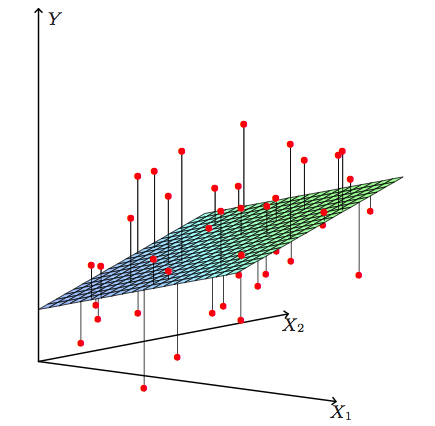
\includegraphics[height=3in]{ols.png}
		\label{fig:ols}
	\end{figure}
\end{frame}


\begin{frame}{Regression as a prediction: Deriving the Algorithm}
	\begin{itemize}
		\item<+-> Denote $\mathbf{X}$ the $N \times (p + 1)$ matrix with each row an input vector (with a 1 in the first position) and $\mathbf{y}$ is the output vector. 
		\item<+-> Write the RSS as:
		$$RSS(\beta) = (\mathbf{y} - \mathbf{X}\beta)^T (\mathbf{y}-\mathbf{x}\beta)$$
		\item<+-> Differentiate with respect to $\beta$:
		\begin{align}
			\frac{\partial\textrm{RSS}}{\partial \beta} &= -2 \mathbf{X}^T(\mathbf{y}-\mathbf{X}\beta)
		\end{align}
		\item<+-> Assume that $\mathbf{X}$ is full rank (no perfect collinearity among any of the independent variables) and set first derivative to 0:
		$$\mathbf{X}^T(\mathbf{y}-\mathbf{X}\beta)=0$$
		\item<+-> Solve for $\beta$:
		$$\hat \beta = (\mathbf{X}^T \mathbf{X})^{-1} \mathbf{X}^T \mathbf{y}$$
	\end{itemize}
\end{frame}


\begin{frame}{Regression as a prediction: Deriving the Algorithm}
\begin{itemize}
\item<+-> What happens if $X$ is not full rank? \pause 
		\textcolor{blue}{There is an infinite number of ways to invert the matrix $X^TX$, and the algorithm does not have a unique solution. There are many values of $\beta$ that satisfy the F.O.C} \\~\\
\item The matrix $X$ is also referred as the design matrix 
\end{itemize}
\end{frame}


\begin{frame}{Regression as a prediction: Making a Prediction}
	\begin{itemize}
\item<+-> The \emph{hat matrix}, or \emph{projection matrix}
		\[ \mathbf{H} = \mathbf{X}(\mathbf{X}^{T}\mathbf{X})^{-1}\mathbf{X}^{T} \text{ with } \mathbf{\tilde{H}} = \mathbf{I} - \mathbf{H} \]
\item<+-> We use the hat matrix to find the fitted values:
		 $$\mathbf{\hat{Y}} = \mathbf{X\hat{\beta}} =\mathbf{ X}(\mathbf{X}^{T}\mathbf{X})^{-1}\mathbf{X}^{T}\mathbf{Y} = \mathbf{HY}$$
\item<+-> We can now write
		\[ \mathbf{e} = (\mathbf{I} - \mathbf{H})\mathbf{Y}  \]
\item<+-> If $\mathbf{HY}$ yields part of $\mathbf{Y}$ that projects into $\mathbf{X}$, this means that $\mathbf{\tilde{H}Y}$ is the part of $\mathbf{Y}$ that does not project into $\mathbf{X}$, which is the \emph{residual} part of $\mathbf{Y}$.  Therefore, $\mathbf{\tilde{H}Y}$ makes the residuals
\item<+-> $\mathbf{e}$ is the part of $\mathbf{Y}$ which is not a linear combination of $X$		
	\end{itemize}
\end{frame}

\begin{frame}{Regression as a prediction: Deriving the Algorithm}
\begin{itemize}
\item Do we make any assumption on the distribution of $\mathbf{Y}$?  \pause  \textcolor{blue}{\textit{No!}}
\pause
\item Can the dependent variable (the response), $\mathbf{Y}$, be a binary variable, i.e $Y \in \lbrace 0,1 \rbrace$?  \pause  \textcolor{blue}{\textit{Yes!}}
\pause
\item Do we assume that homoskedasticity, i.e that $Var(Y_i)=\sigma^2$, $\forall_i$?   \pause \textcolor{blue}{\textit{No!}}
\pause
\item Is the residuals, $\mathbf{e}$, correlated with $\mathbf{Y}$? Do we need to make any additional assumption in order for $corr(\mathbf{e},\mathbf{X})=0$?  \pause \textcolor{blue}{\textit{No!} The OLS algorithm will always yield residuals which are not correlated with the covariates}
\pause
\item The procedure we discussed so far is an algorithm, which solves an optimization problem (minimizing a square loss function). The algorithm requires an assumption of full rank in order to yield a unique solution, however it does not require any assumption on the distribution or the type of the response variable, $\mathbf{Y}$ 
\end{itemize}
\end{frame}

%\begin{frame}{Regression as a prediction}
%\begin{itemize}
%\item 
%\end{itemize}
%\end{frame}


\begin{frame}{Regression as a model: From algorithm to model}
\begin{itemize}
\item<+-> Now we make stronger assumptions, most importantly we assume a data generating process (hence DGP), i.e we assume a functional form for the relationship between $Y$ and $X$ \\~\\
%\item<+-> \emph{Linear in Parameters}: $Y$ is related to the independent variables and the error term as $Y = X\beta + \epsilon$
\item<+-> Is $Y$ a linear function of the covariates? 
\pause \textcolor{blue}{\textit{No}, it is a linear function of $\beta$} \\~\\
\item<+-> What are the classic assumptions of the regression model?
\end{itemize}
\end{frame}

\begin{frame}{Regression as a model: The classic assumptions of the regression model}
\begin{enumerate}
\item The dependent variable is linearly related to the coefficients of the model and the model is correctly specified,
$Y = X\beta + \epsilon$
\item The independent variables, $X$, are fixed, i.e are not random variables (this can be relaxed to $Cov(X,\epsilon)=0$)
\item The conditional mean of the error term is zero, 
$\mathbb{E}(\epsilon|X)=0$ 
\item Homoscedasticity. The error term has a constant variance, i.e $\mathbb{V}(\epsilon_i)=\sigma^2$ 
\item  The error terms are uncorrelated with each other, $Cov(\epsilon_i, \epsilon_j) = 0$
\item The design matrix, $X$, has full rank
\item The error term is normally distributed, i.e $\epsilon \sim N(0,\sigma^2)$ (the mean and variance follows from (3) and (4))
\end{enumerate}
\end{frame}

\begin{frame}{Discussion of the classic assumptions of the regression model}
\begin{itemize}
\item The assumption that $\mathbb{E}(\epsilon|X)=0$ will always be satisfied when there is an intercept term in the model, i.e when the design matrix contains a constant term \pause
\item When $X\perp \epsilon$ it follows that $Cov(X,\epsilon)=0$ \pause
\item  The normality assumption of $\epsilon_i$ is required for hypothesis testing on $\beta$ \pause \\
The assumption can be relaxed for sufficiently large sample sizes, as by the CLT, $\hat{\beta}_{OLS}$ converges to a normal distribution when 
$N\rightarrow \infty$. What is a sufficiently large sample size? 
\end{itemize}
\end{frame}

\begin{frame}{Properties of the OLS estimators: Unbiased estimator}
The OLS estimator of $\beta$ is,
	%when plugging in Xbeta + epsilon, make sure to say that that is the true model...
	\begin{align*}
	 \hat{\beta} &= (X^{T}X)^{-1}X^{T}Y\\
				 &= (X^{T}X)^{-1}X^{T}(X\beta + \epsilon) \\
				 &= (X^{T}X)^{-1}X^{T}X\beta + (X^{T}X)^{-1}X^{T}\epsilon \\
				 &= \beta + (X^{T}X)^{-1}X^{T}\epsilon 
	\end{align*}
	We know that $\hat{\beta}$ is unbiased if $E (\hat{\beta}) = \beta$

	\[ \begin{array}{rl}
	E (\hat{\beta}) &= E(\beta + (X^{T}X)^{-1}X^{T}\epsilon | X) \\
	 &= E(\beta | X) + E((X^{T}X)^{-1}X^{T}\epsilon | X) \\
	 &= \beta + (X^{T}X)^{-1} E(\epsilon | X) \\
	 &\qquad \text{where } E(\epsilon | X) = E(\epsilon) = 0 \\
	E (\hat{\beta}) &= \beta 
	\end{array} \]
\end{frame}

\begin{frame}{Properties of the OLS estimators: Unbiased estimator}
\begin{itemize}
\item What assumptions are used for the proof that $\hat{\beta}_{OLS}$ is an unbiased estimator?\\  \pause
\textcolor{blue}{Assumption (1), the model is correct. \\
Assumption (2), the covariates are independent of the error term}
\end{itemize}
\end{frame}

\begin{frame}[t]\frametitle{Properties of the OLS estimators: The variance of $\hat{\beta}_{OLS}$}
	\begin{itemize}
		\item Recall:				
			\[ \begin{array}{rrl} & \hat{\beta} &= (X^{T}X)^{-1}X^{T}Y \nonumber \\
			& &= (X^{T}X)^{-1}X^{T}(X\beta + \epsilon) \\
			\Rightarrow & \hat{\beta} - \beta &= (X^{T}X)^{-1}X^{T} \epsilon
			\end{array} \]
			\item Plugging this into the covariance equation:
			\[ \begin{array}{rl}
			cov(\hat{\beta} | X) &= E[(\hat{\beta} - \beta)(\hat{\beta} - \beta)'|X] \\
			 &= E\big[ \big((X^{T}X)^{-1}X^{T}\epsilon \big) \big((X^{T}X)^{-1}X^{T}\epsilon)' | X\big] \\
			 &= E[ (X^{T}X)^{-1}X^{T} \epsilon \epsilon^{T}X(X^{T}X)^{-1} | X] \\
			 &= (X^{T}X)^{-1}X^{T} E(\epsilon\epsilon^{T} | X) X(X^{T}X)^{-1}  \\
			 &\qquad \text{where } E(\epsilon\epsilon^{T} | X) = \sigma^{2} I_{p \times p} \\
			 &= (X^{T}X)^{-1}X^{T} \sigma^{2} I_{p \times p} X(X^{T}X)^{-1} \\
			&= \sigma^{2} (X^{T}X)^{-1}X^{T}X(X^{T}X)^{-1} \\
			&= \sigma^{2} (X^{T}X)^{-1}
			\end{array} \]
	\end{itemize}
	\end{frame}

\begin{frame}{Estimating $\sigma^2$}
We estimate $\sigma^2$ by dividing the residuals squared by the degrees of freedom because the $e_{i}$ are generally smaller than the $\epsilon_{i}$ due to the fact that $\hat{\beta}$ was chosen to make the sum of square residuals as small as possible.
		$$ \hat{\sigma}_{OLS}^2 = \frac{1}{n-p}\sum_{i = 1}^{n} e_{i}^2 $$ 
\pause
Compare the above estimator to the classic variance estimator: 
$$ \hat{\sigma}_{classic}^2 = \frac{1}{n-1}\sum_{i = 1}^{n} \left( Y_i -\bar{Y} \right)^2 $$
\pause
Is one estimator always preferable over the other? If not when each estimator is preferable?
\end{frame}


\begin{frame}[fragile]{measurment error}
Consider the following DGP (data generating process):
\begin{verbatim}
n=200
x1 = rnorm(n,mean=10,1)
epsilon = rnorm(n,0,2)
y = 10+5*x1+epsilon

### mesurment error:
noise = rnorm(n,0,2)
x1_noise = x1+noise
\end{verbatim}
The true model has $x_1$, however we observe only $x_1^{noise}$. We will investigate the effect of the noise and the distribution of the noise on the OLS estimation of $\beta_1$. The true value of the parameter of interest is, $\beta_1 = 5$ 
\end{frame}

\begin{frame}{Measurement error: $noise \sim N(\mu = 0,\sigma = 2)$}
\begin{figure}
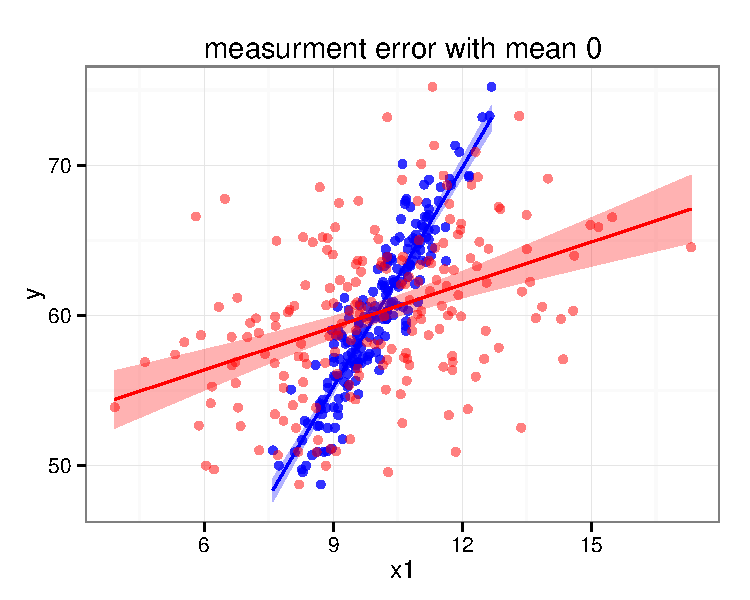
\includegraphics[scale=0.8]{ols1.pdf}
\end{figure}
\end{frame}

\begin{frame}{Measurement error: $noise \sim N(\mu = 5,\sigma = 2)$}
\begin{figure}
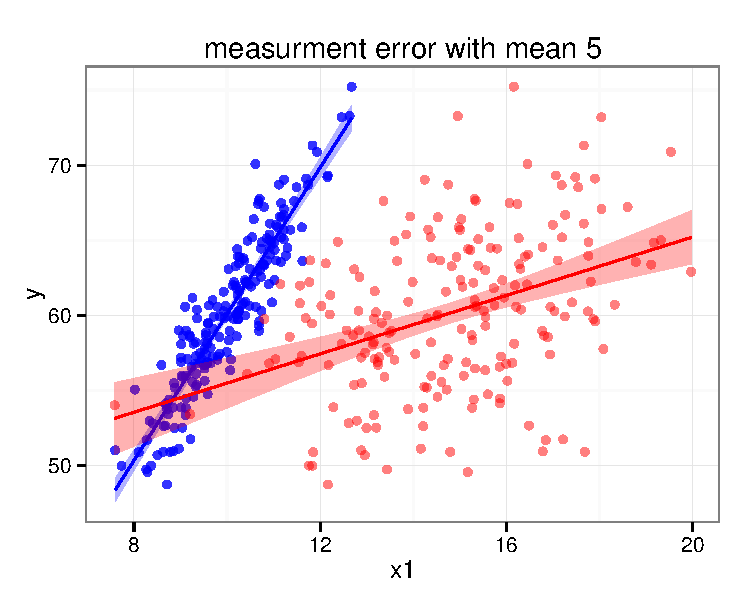
\includegraphics[scale=0.8]{ols2.pdf}
\end{figure}
\end{frame}

\begin{frame}{Measurement error: $noise \sim N(\mu = ?,\sigma = 2)$}
\begin{figure}
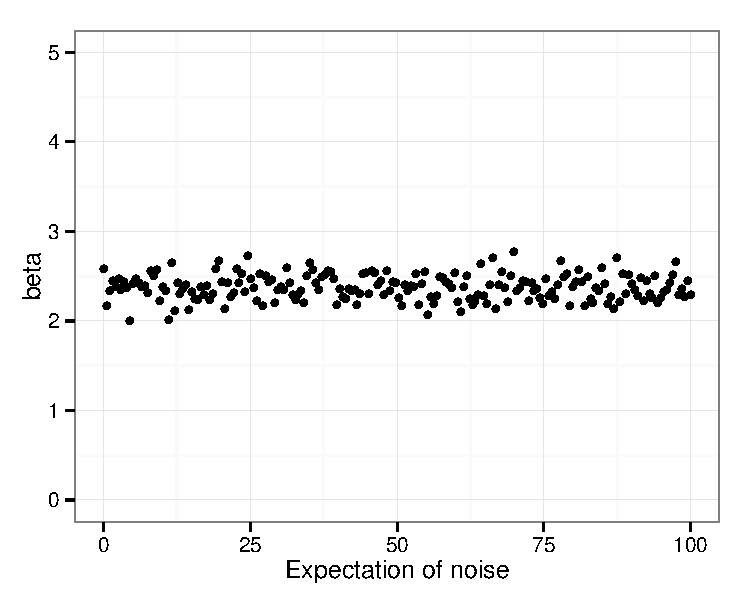
\includegraphics[scale=0.8]{ols4.pdf}
\end{figure}
\end{frame}

\begin{frame}{Measurement error: $noise \sim N(\mu = 5,\sigma = ?)$}
\begin{figure}
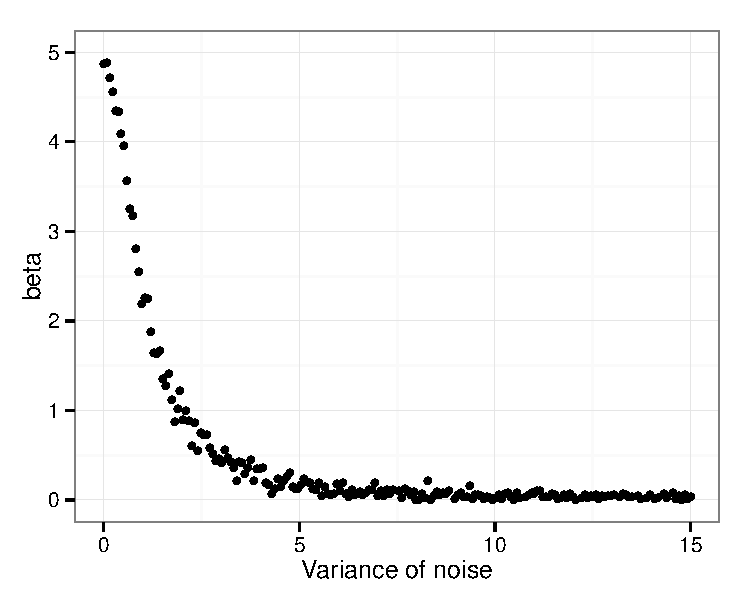
\includegraphics[scale=0.8]{ols3.pdf}
\end{figure}
\end{frame}

\begin{frame}{Measurement error: $noise \sim exp(\lambda = ?)$}
\begin{figure}
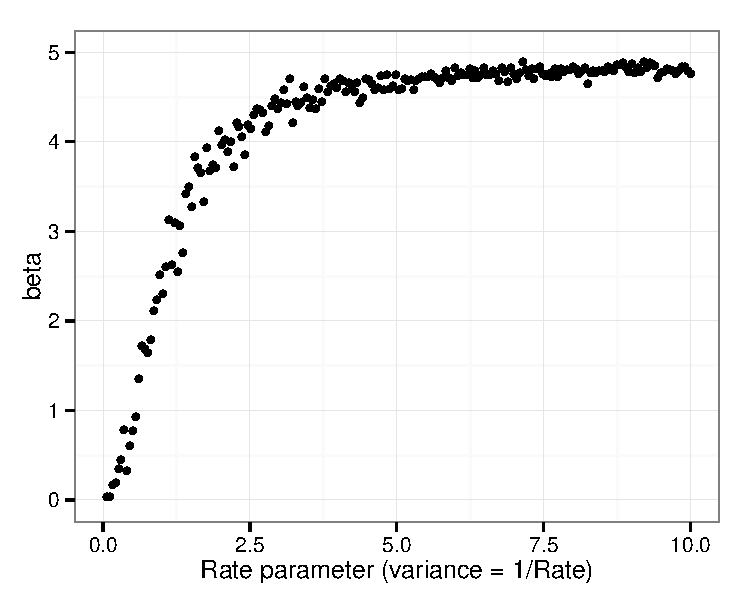
\includegraphics[scale=0.8]{ols5.pdf}
\end{figure}
\end{frame}

\begin{frame}{Measurement error}
\begin{itemize}
\item Could we reach the same conclusions as the simulations from analytical derivations?\pause
\textcolor{blue}{\textit{Yes}}
\item As we saw before,
$$ \mathbb{E}(\hat{\beta}_{OLS}) = \frac{Cov(y,x_1^{noise})}{\mathbb{V}(x_1^{noise})} 
 = \frac{Cov(y,x_1+noise)}{\mathbb{V}(x_1+noise)}$$
 $$ = \frac{Cov(y,x_1)}{\mathbb{V}(x_1)+\mathbb{V}(noise)}$$
 \pause
 Therefore as $\mathbb{V}(noise)\rightarrow \infty$, the expectation of the OLS estimator of $\beta$ will converge to zero,
 $$\mathbb{V}(noise)\rightarrow \infty \Rightarrow \mathbb{E}(\hat{\beta}_{OLS}) = \frac{Cov(y,x_1)}{\mathbb{V}(x_1)+\mathbb{V}(noise)} \rightarrow 0$$
\end{itemize}
\end{frame}

\begin{frame}[fragile]{Measurement error in the dependent variable}
\begin{itemize}
\item Consider the situation in which $y_i$ is not observed, but $y_i^{noise}$ is observed. There are no measurement error in $x_1$. 
\item The model (DGP) is,
\[ y_i = 10+5*x_{1i}+\epsilon_i \]
\[ y_i^{noise} = y_i+noise_i \]
\item Will the OLS estimator of $\beta_1$ be unbiased? \pause \textcolor{blue}{Yes}
\[
\mathbb{E}(\hat{\beta}_{OLS}) = \frac{Cov(y^{noise},x_1)}{\mathbb{V}(x_1)} 
 = \frac{Cov(y+noise,x_1)}{\mathbb{V}(x_1)}\] 
\[ = \frac{Cov(y,x_1)}{\mathbb{V}(x_1)} = \beta_1
\]
\item This model is equivalent to the model, $y_i = 10+5*x_{1i}+(\epsilon_i+noise_i) $, where $y_i$ is observed. 
\end{itemize}
\end{frame}

\begin{frame}[fragile]{Measurment error in the dependent variable}
\begin{itemize}
\item Will the OLS estimator be unbiased if the measurement error was multiplicative instead of additive? Formally, if the DGP was:
\[ y_i = 10+5*x_{1i}+\epsilon_i \]
\[ y_i^{noise} = y_i \cdot noise_i \] \pause
\item Analytic derivations:
\[
\mathbb{E}(\hat{\beta}_{OLS}) = \frac{Cov(y^{noise},x_1)}{\mathbb{V}(x_1)} 
 = \frac{Cov(y \cdot noise,x_1)}{\mathbb{V}(x_1)}\] 
\pause
\[ Cov (y \cdot noise,x_1) = \mathbb{E}(y \cdot noise \cdot x_1) - 
\mathbb{E}(y \cdot noise) \cdot \mathbb{E}(x_1) \]
\[ = \frac{\mathbb{E}(noise) \cdot Cov(y,x_1)}{\mathbb{V}(x_1)}
 =  \mathbb{E}(noise) \cdot \beta_1\] 
\end{itemize}
\end{frame}

\begin{frame}[fragile]{Measurment error in the dependent variable}
\textit{When there is multiplicative noise the bias of $\hat{\beta}$ is influenced by $\mathbb{E}(noise)$, not from $\mathbb{V}(noise)$}

% Need to add the numbers from the simulation and a plot
\end{frame}



\begin{frame}{Gauss-Markov theorem: BLUE}
\begin{itemize}
\item The regression estimator is a linear estimator, $\hat{\beta} = Cy$, where $C = (X^T X)^{-1}X^T$. A linear estimator is any $\hat{\beta_j}$ such that 
$\hat{\beta_j} = c_1y_1+c_2y_2+\dots+c_py_p$ \\~\\

\item The Gauss-Markov theorem: If assumptions: (2),(3),(4),(5) hold. The regression estimator is the best linear unbiased estimator (BLUE), in terms of MSE (Mean Squared Error)  
\end{itemize}
\end{frame}

\begin{frame}{Frisch-Waugh-Lovell: Regression Anatomy}
\begin{itemize}
\item<+-> In the simple bivariate case:
		 $$\beta_1=\frac{\textrm{Cov}(Y_i,X_i)}{\textrm{Var}(X_i)}$$
 \item<+-> In the multivariate case, $\beta_j$ is:
		$$\beta_j=\frac{\textrm{Cov}(Y_i,\tilde{X}_{ij})}{\textrm{Var}(\tilde{X}_{ij})}$$
where $\tilde{X}_{ij}$ is the residual from the regression of $X_{ij}$ on all other covariates.
\item<+-> The multiple regression coefficient $\hat \beta_j$ represents the additional contribution of $x_j$ on $y$, after $x_j$ has been adjusted for $1, x_1, \dots, x_{j-1}, x_{j+1}, \dots, x_p$ 
\item<+-> What happens when $x_j$ is highly correlated with some of the other $x_k$'s?
\end{itemize}
\end{frame}

\begin{frame}{Frisch-Waugh-Lovell: Regression Anatomy}
\begin{itemize}
\item<+-> Claim: $\beta_j =\frac{\textrm{Cov}(\tilde{Y_i},\tilde{X}_{ij})}{\textrm{Var}(\tilde{X}_{ij})}$, i.e $Cov(Y_i,\tilde{X_{ij}})=
Cov(\tilde{Y_i},\tilde{X_{ij}})$ 
\item<+-> Proof:\\
 Let $\tilde{Y_{i}}$ be the residuals of a regression of all the covariates except $X_{ji}$ on $Y_{i}$, i.e
 \[ X_{ji} = \beta_0 +\beta_1 X_{1i} +\beta_2 X_2+\dots+\beta_P X_{Pi}+f_i\] 
\[ Y_{i} = \alpha_0 +\alpha_1 X_{1i} +\alpha_2 X_2+\dots+\alpha_P X_{Pi}+e_i\] 
Then, $\hat{e}_i = \tilde{Y_{i}}$, and $\hat{f}_i = \tilde{X_{ji}}$
\item<+-> It follows from the OLS algorithm that $Cov(x_{ki},\tilde{X_{ji}})=0,\; \forall_{k\neq j}$. As the residuals of a regression are not correlated with any of the covariates \pause

\[ Cov(\tilde{Y_i},\tilde{X_{ij}}) =  
Cov(Y_i - \hat{\alpha}_0 -\hat{\alpha}_1 X_{1i} -\hat{\alpha}_2 X_2-\dots+\hat{\alpha}_P X_{Pi},\tilde{X_{ij}}) \]
\[ =  Cov(Y_i,\tilde{X_{ij}})\]

%\pause \textcolor{blue}{Yes}
\end{itemize}
\end{frame}

\begin{frame}{Asymptotics of OLS }
\begin{itemize}
\item Is the OLS estimator of $\beta$ consistent? \pause \textcolor{blue}{Yes}
\item Proof:
\item Denote the observed characteristics of observation $i$ by $x_i$. What is the dimensions of $x_i$?
\pause \textcolor{blue}{$1 \times p$}   
\item $x_i = (x_{i1},x_{i2},\dots,x_{ip})$ and 
$ x_i^T = \left(  \begin{array}{c}
x_{i1} \\
x_{i2} \\
\vdots \\
x_{ip}
\end{array} \right)$
\pause
\item  
 $ x_i^T x_i = \left(
\begin{array}{cccc}
x_{i1}^2 & x_{i1}x_{i2} & \dots & x_{i1} x_{ip} \\
x_{i2} x_{i1} & x_{i2}^2 & \dots & x_{i2} x_{ip} \\
\vdots & \vdots & \vdots &  \\
x_{ip} x_{i1} & x_{ip} x_{i2} & \dots & x_{ip}^2 
\end{array} \right)
$
\end{itemize}
\end{frame}


\begin{frame}{Asymptotics of OLS }
\begin{itemize}
\item Verify at home that, 
 \[ X^T X = \left(
\begin{array}{cccc}
\sum_{i=1}^n x_{i1}^2 & \sum_{i=1}^n x_{i1}x_{i2} & \dots & \sum_{i=1}^n x_{i1} x_{ip} \\
\sum_{i=1}^n x_{i2} x_{i1} & \sum_{i=1}^n x_{i2}^2 & \dots & \sum_{i=1}^n x_{i2} x_{ip} \\
\vdots & \vdots & \vdots &  \\
\sum_{i=1}^n x_{ip} x_{i1} & \sum_{i=1}^n x_{ip} x_{i2} & \dots & \sum_{i=1}^n x_{ip}^2 
\end{array} \right)_{(p \times p)}
\]
\pause
\item Hence, $X^T X = \sum_{i=1}^n x_{i}^T x_{i}$
\item Note (and verify at home), 
\[ X^T y = 
\left( \begin{array}{c}
\sum_{i=1}^n x_{i1} y_i  \\
\sum_{i=1}^n x_{i2} y_i  \\
\vdots  \\
\sum_{i=1}^n x_{ip} y_i
\end{array} \right) 
= \sum_{i=1}^n x_i^T y_i \]
\end{itemize}
\end{frame}

\begin{frame}{Asymptotics of OLS }
\begin{itemize}
\item The OLS estimator is, $\beta = \left( X^TX \right)^{-1} X^T y$
\item Recall $\left( X \cdot k \right)^{-1} = k^{-1} \cdot \left( X \right)^{-1}$
\item Multiplying and dividing by $\frac{1}{n}$ yields, 
$$\beta = \left( \frac{1}{n} X^TX \right)^{-1} \left( \frac{1}{n} X^T y \right) 
= \left( \frac{1}{n} \sum_{i=1}^n x_i^T x_i \right)^{-1} \left( \frac{1}{n} \sum_{i=1}^n x_i^T y_i \right)$$

\[ \rightarrow \mathbb{E}\left(x_i^T x_i\right)^{-1}\cdot \mathbb{E}\left( x_i^T y_i\right) 
 = \mathbb{E}\left(x_i^T x_i\right)^{-1}\cdot \mathbb{E}\left( x_i^T \left(x_i \beta + \epsilon_i \right) \right) \]
\item The converges follows from the central limit theorem (CLT). 
\[ = \mathbb{E}\left(x_i^T x_i\right)^{-1} \cdot \mathbb{E}\left( x_i^T x_i\right) \beta
+\mathbb{E}\left(x_i^T x_i\right)^{-1} \cdot \mathbb{E}\left( x_i^T \epsilon_i\right) = \beta \] 
\end{itemize}
\end{frame}


\begin{frame}{Regression in  Causal Analysis}
	\begin{itemize}
\item Imagine we are analyzing a \emph{randomized} experiment with a regression using the following model:
		$$Y_i=\alpha + \beta_1 \cdot T_i + \mathbf{X}^T_i\cdot \mathbf{\beta}_2+\epsilon_i$$
		where $T_i$ is an indicator variable for treatment status and $\mathbf{X}_i$ is a vector of \emph{pre-treatment characteristics}
\item<+-> Under this model, what is random?  
%\item<+-> How do we interpret the coefficients on $\mathbf{X}_i$?
\item<+-> How do we interpret the coefficient  $\beta_1$? 
	\end{itemize}
\end{frame}
































\end{document}